\chapter{Theoretical Framework}
\label{chapter:theoretical-framework}


This chapter describes the theoretical concepts needed to understand the work that will be developed during the research's execution.


\section{FER}

Facial Expression Recognition (FER) is a crucial area of research in affective computing and human-computer interaction. It involves detecting and classifying human emotions based on facial expressions, which can enhance applications in psychology, security, and social robotics. Traditional FER methods relied on handcrafted features, such as Local Binary Patterns (LBP) and Histogram of Oriented Gradients (HOG), but deep learning has significantly advanced the field. Convolutional Neural Networks (CNNs) and Vision Transformers (ViTs) have demonstrated superior performance in FER by learning hierarchical spatial features and capturing global dependencies, respectively  \cite{zheng_poster_2022}, \cite{kollias_affect_2021}. 

Despite these advancements, FER remains challenging due to variations in lighting, occlusions \cite{guo_occrob_2023}, and individual differences in expressing emotions. Datasets such as AffectNet, FER2013, and RAF-DB have been instrumental in training robust models, but their annotations introduce inherent subjectivity. RAF-DB provides diverse in-the-wild facial expressions, making it valuable for evaluating model robustness. This has led to growing interest in improving the robustness of FER architectures, particularly through modifications in model heads and multi-layer perceptrons (MLPs) to enhance generalization and representation learning \cite{abdullah_activator_2024},\cite{yu_rethinking_2021}. 

Recent research has also explored multimodal approaches that incorporate voice and physiological signals to complement facial expressions for example Zhao et al. \cite{zhao_former-dfer_2021}. These hybrid systems aim to enhance recognition accuracy by providing additional context to emotion classification, reducing ambiguity caused by facial occlusions or partial expressions \cite{wang_survey_2024}. Future work may focus on integrating cross-modal transformers that efficiently fuse information from multiple techniques to improve FER performance. 

\subsection{Emotional Labeling}

Emotions are commonly categorized using two main approaches: discrete classification and dimensional models. Paul Ekman’s six basic emotions (happiness, sadness, fear, disgust, surprise, and anger) have been widely adopted in FER, but alternative theories, such as the circumplex model, represent emotions along valence and arousal dimensions \cite{russell_circumplex_1980}. The choice of labeling affects model performance, as categorical approaches simplify recognition but may fail to capture nuanced emotional states \cite{mollahosseini_affectnet_2019}, \cite{kollias_affect_2021}. 

Labeling in FER datasets is often noisy due to human subjectivity, inter-annotator disagreements, and cultural differences in emotional expression. Researchers have explored semi-supervised learning and self-supervised techniques to mitigate these issues by leveraging large-scale unlabeled data (Zhang et al., 2022 \cite{zhang_transformer-based_2022}). Additionally, multi-label approaches are gaining traction, allowing for more flexible emotion representation and improving generalization in real-world applications. 

Advancements in synthetic data generation have also been explored to address labeling challenges. Techniques such as Generative Adversarial Networks (GANs) and Variational Autoencoders (VAEs) have been used to generate high-fidelity facial expressions, providing additional labeled training data and improving the robustness of FER models to diverse emotional expressions. 

\subsection{FER in-the-wild}

FER in controlled environments, such as laboratory settings, differs significantly from real-world ("in-the-wild") scenarios, where factors like illumination changes, occlusions, and spontaneous expressions impact model performance. In-the-wild datasets, including AffectNet, RAF-DB, and ExpW, provide diverse samples that improve model robustness but also introduce challenges like class imbalance and mislabeled data \cite{zhang_leave_2023}. 


\begin{figure}[H]
\centering
   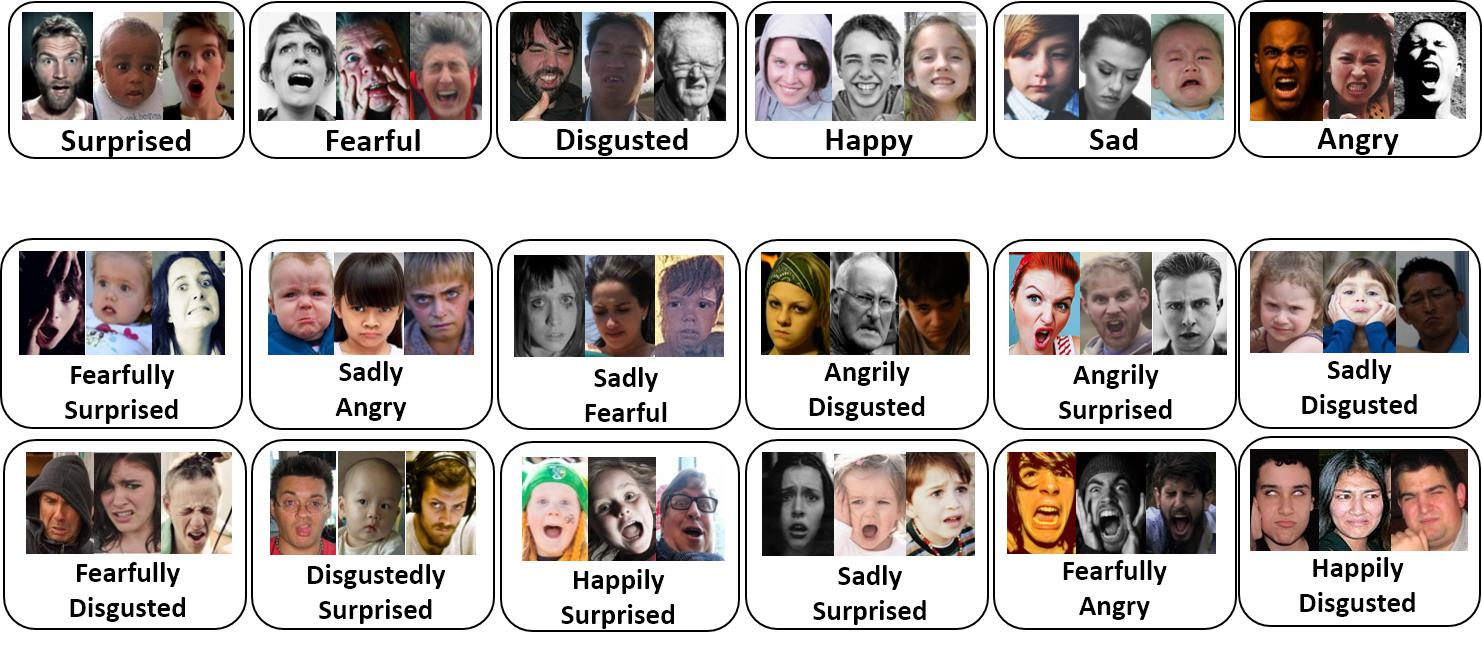
\includegraphics[width=0.70\textwidth]{../images/faces_rafdb_dataset.png}
\caption{Real-world Affective Faces Database (RAF-DB), dataset for facial expression}
\label{fig:RAF-DB}
\end{figure}

 
Recent works have incorporated domain adaptation, batch attention and contrastive learning to enhance in-the-wild FER. Transfer learning from large-scale vision models, such as ViTs, has proven effective in improving generalization to unseen expressions for example Her et al \cite{her_batch_2024}. However, real-time performance remains an issue, prompting researchers to investigate efficient architectures and explore new techniques to deploy FER models on edge devices.


Another emerging approach involves leveraging facial dynamics rather than static images. Temporal modeling techniques, such as graph convolutional networks (GCNs) and optical flow analysis, have been proposed to enhance in-the-wild FER by capturing motion-based cues \cite{wang_survey_2024}. These approaches improve robustness to varying facial conditions and enable more accurate emotion recognition in real-world applications. 

\section{FER Architectures}


\subsection{Deep Learning for FER}

Deep learning has revolutionized FER by replacing handcrafted features with automatically learned representations. CNNs, such as VGG-16, ResNet, and EfficientNet \cite{tan_efficientnet_2020}, have demonstrated strong performance by capturing spatial hierarchies within facial images. Recent approaches have leveraged hybrid architectures, combining CNN feature extractors with recurrent neural networks (RNNs) or attention mechanisms to better model temporal dynamics in video-based FER for example Dosovitskiy et al. 2021 \cite{dosovitskiy_image_2021} 

However, CNN-based models struggle with long-range dependencies, leading to interest in transformer architectures. These models, originally designed for natural language processing, have shown promise in capturing complex spatial relationships in facial expressions. 

\subsection{Visual Transformer}

The shift towards transformers has opened new avenues for improving FER, particularly by modifying their classification heads and MLP layers to enhance discriminative power.  One such model is POSTER: A Pyramid Cross-Fusion Transformer Network for Facial Expression Recognition, which introduces a hierarchical fusion mechanism to enhance local and global facial feature interactions. POSTER effectively balances efficiency and accuracy by integrating multi-scale information processing within a transformer framework, demonstrating superior performance on benchmark FER datasets \cite{zheng_poster_2022}.

POSTER addresses intra-class variation by leveraging a pyramid structure for multi-scale feature extraction, ensuring robust representation of subtle differences within the same expression. Its cross-fusion mechanism refines feature interactions, reducing the impact of pose, lighting, and intensity variations while enhancing consistency. To tackle inter-class variation, POSTER employs attention-based differentiation and hierarchical refinement, helping distinguish similar expressions by focusing on key distinguishing features. 

\begin{figure}[H]
\centering
   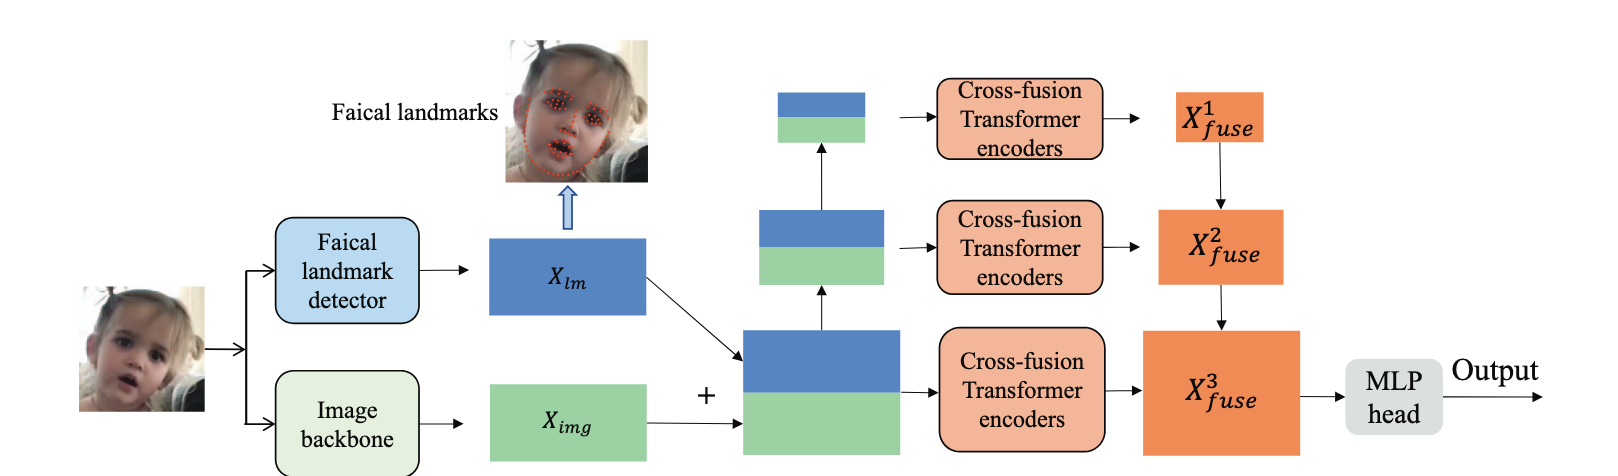
\includegraphics[width=0.70\textwidth]{../images/poster_image.png}
\caption{POSTER Cross-Fusion Transformer Arquitecture Example}
\label{fig:poster_architecure_example}
\end{figure}


\begin{figure}[H]
\centering
   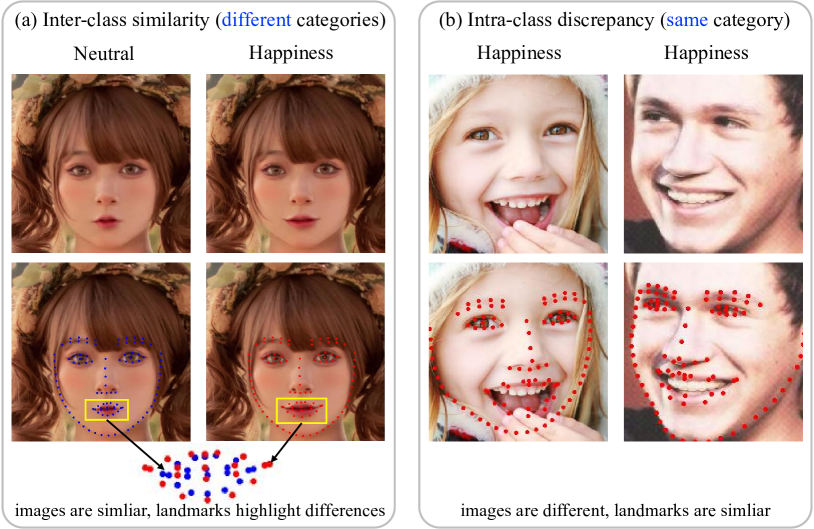
\includegraphics[width=0.70\textwidth]{../images/intra_inter_classes_images.png}
\caption{POSTER Cross-Fusion Transformer Intra and Inter Image Classes}
\label{fig:intra_inter_classes_images}
\end{figure}
	
\begin{figure}[H]
\centering
   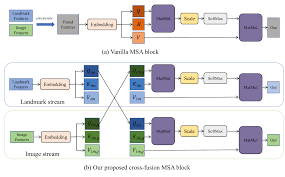
\includegraphics[width=0.70\textwidth]{../images/poster_cross_function.png}
\caption{POSTER Cross-Fusion Transformer vs Previous Versions}
\label{fig:poster_cross_function}
\end{figure}
	

Self-supervis

Self-supervised learning techniques have also gained popularity in FER, as develop by Park et al\cite{park_what_2023}. These methods are particularly beneficial because they allow models to learn meaningful facial representations from large amounts of unlabeled data, reducing dependence on expensive annotated datasets. Given the inherent subjectivity and variability in emotional expressions, self-supervised learning helps improve generalization by capturing robust feature representations across different demographics, lighting conditions, and occlusions. Techniques such as contrastive learning and clustering-based approaches have demonstrated significant improvements in adaptability and performance for FER tasks. By leveraging unlabeled datasets, models can learn meaningful facial representations without explicit supervision, reducing the reliance on large annotated datasets. 



\section{FER Performance and Evaluation}


\subsection{Performance Metrics for FER}

Evaluating FER models requires appropriate performance metrics that capture both classification accuracy and robustness. Unlike other computer vision tasks, FER must contend with subtle variations in facial expressions, subjective emotion labels, and real-world challenges such as occlusions and lighting changes. These factors make robustness particularly critical, as models need to generalize well across diverse populations, emotional intensities, and environmental conditions. Standard metrics include accuracy, precision, recall, and F1-score, with the latter being particularly useful for handling class imbalances in datasets like RAF-DB and AffectNet. Additionally, area under the curve (AUC) and confusion matrices help assess model reliability across different emotional categories \cite{ma_facial_2023}.

One challenge in FER evaluation is the subjective nature of emotional labels, which can lead to misclassifications even in well-performing models. Researchers have proposed leveraging uncertainty estimation techniques and human-in-the-loop approaches to refine model predictions and enhance interpretability. Moreover, explainability methods, such as Grad-CAM and attention visualization, provide insights into how FER models make predictions, increasing their trustworthiness.

Cross-dataset evaluations have also become an essential aspect of FER benchmarking. For example, a study by Ma et. 2024 \cite{ma_facial_2023} evaluated a transformer-based FER model trained on AffectNet and tested on RAF-DB, highlighting the challenges of domain shifts and variations in emotional expression. Such studies emphasize the necessity of developing FER models that generalize well across datasets with different annotation styles, demographic distributions, and environmental conditions. Cross-dataset evaluations help identify robustness gaps and encourage the design of architectures that are more resilient to dataset biases. Evaluating models across multiple datasets ensures that they generalize well beyond their training domain, addressing issues related to dataset bias and overfitting. 

Another key evaluation metric is Mean Average Precision (mAP)  used in object detection and retrieval tasks, assessing a model’s ability to accurately predict object locations and classifications. It is derived from the Precision-Recall (PR) curve, where precision measures how many predicted objects are correct, and recall measures how many actual objects are detected. The metric computes the Average Precision (AP) for each object class, which represents the area under the PR curve, and then averages these AP scores across all classes\cite{marcu_pitfalls_2022} \cite{ranjan_light-weight_2018}.

\subsection{Evaluation of Modified Heads}

The evaluation of modified heads in FER architectures plays a crucial role in determining their impact on recognition accuracy and robustness. Model heads, particularly the multi-layer perceptrons (MLPs) used in transformer-based FER models, influence the ability to capture and classify facial features effectively. By modifying these heads, researchers aim to enhance feature representations and improve performance on benchmark datasets such as RAF-DB and AffectNet \cite{zheng_poster_2022}.

One approach involves introducing adaptive MLP layers that incorporate attention mechanisms or gating functions to refine extracted features before classification. Such modifications have been shown to improve generalization, especially in in-the-wild FER scenarios where facial expressions vary significantly due to real-world conditions. Experimental studies indicate that evaluating modified heads using cross-validation techniques and ablation studies helps identify their effectiveness in different settings \cite{abdullah_activator_2024}.

Furthermore, integrating auxiliary loss functions or regularization techniques within modified heads can prevent overfitting and improve model interpretability. Researchers have explored loss functions tailored for imbalanced emotional categories, ensuring better recognition across underrepresented emotions. As FER continues to advance, optimizing and evaluating these architectural modifications will remain a key area of research.


%\section{Concept 1}
%
%\label{section:Concept1}
%
%First theoretical framework concept goes here.
%
%\subsection{Subsection of Concept 1} 
%\subsection{Subsection 2 of Concept 1}
%Some text goes here \cite{examplereference}. An example of displaying and referencing an image is shown in \textbf{Figure \ref{fig:example}}
%
%
%\begin{figure}
%	\begin{center}
%		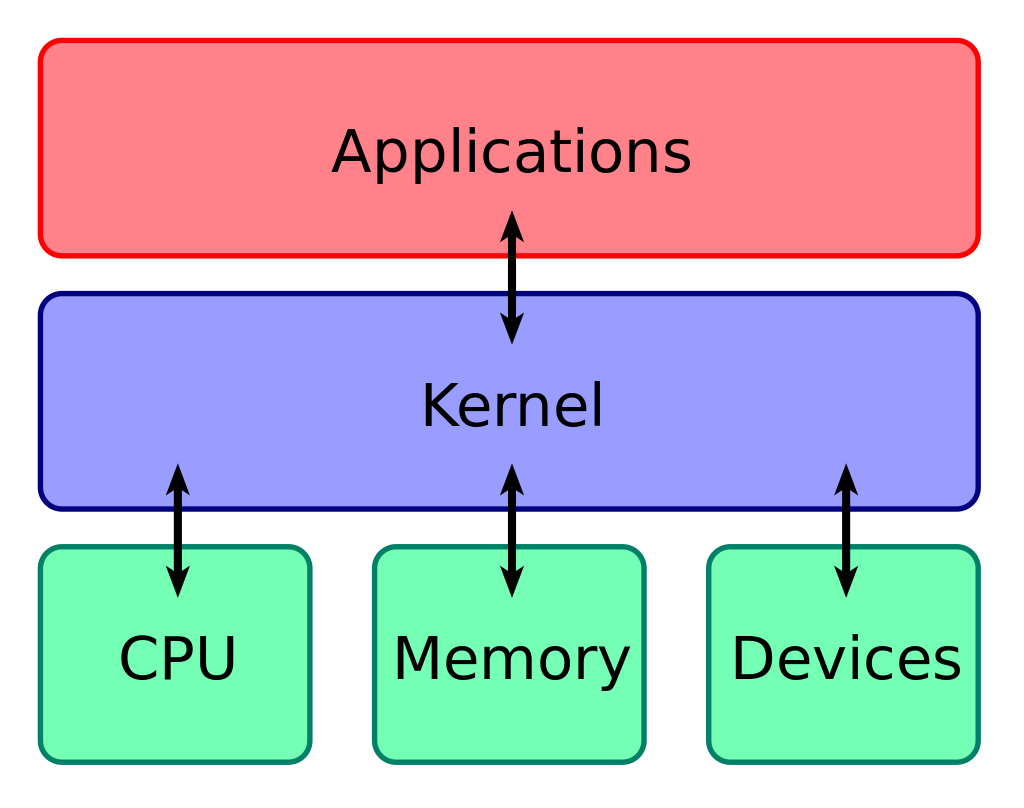
\includegraphics[width=1\columnwidth]{../img/image.png}
%		\caption[]{Example image with reference \cite{examplereference}.}
%		\label{fig:example}
%	\end{center}
%\end{figure}
%
%
%\section{Concept 2}
%
%\label{section:Concept2}
%
%\subsection{Subsection Concept 2}
%
%\subsubsection{Subsection 2 Concept 2}
%
%\section{Concept 3}
%An example of pseudo-code can be seen in \textbf{Algorithm \ref{examplepseudocode}}
%
%\begin{pseudocode}{Pseudo\_Code}{Input} \label{examplepseudocode}
%	\FOR y \GETS 1 \TO Input.MaxL \DO
%	\BEGIN
%	\FOR x \GETS 1 \TO Input.MaxH \DO
%	\BEGIN
%	a \GETS \CALL {FunctionCall}{x,y}\\
%	b \GETS \CALL {AnotherFunction}{x, y}\\
%	\CALL {ThirdFunction}{a,b}
%	\END
%	\END
%\end{pseudocode}
%
%
%\subsection{Example equation}
% Equation \ref{eq:1} shows an example equation.
%
%\[
%I=(L\cdot N) \tag{1} \label{eq:1}
%\]
  
\section{Related Work}
The related work for the research is include in this section:

Facial expression recognition (FER) has been extensively studied over the past decades, evolving from traditional machine learning approaches to deep learning methods. Early FER systems relied on handcrafted features such as Local Binary Patterns (LBP) and Histogram of Oriented Gradients (HOG). These approaches, while computationally efficient, often struggled to generalize across diverse datasets due to limited feature representation capabilities. 

The advent of convolutional neural networks (CNNs) revolutionized FER by enabling automatic feature extraction, with architectures such as VGGNet, ResNet \cite{he_deep_2015}, and EfficientNet achieving significant performance improvements. However, CNNs face limitations in capturing global dependencies and spatial relationships in images, which has motivated the exploration of transformer-based models in computer vision tasks \cite{islam_recent_2023}.

The introduction of Vision Transformers (ViTs) by Dosovitskiy \cite{dosovitskiy_image_2021} marked a significant shift in how visual tasks are approached. By leveraging self-attention mechanisms, ViTs can model long-range dependencies and capture richer contextual information compared to traditional CNNs.


In recent work on Facial Expression Recognition (FER), several models have demonstrated promising results, each with its unique strengths and limitations. ResNet-50 \cite{he_deep_2015} , a baseline convolutional neural network (CNN), performs well in local feature extraction, achieving an accuracy of 86.34\%. However, it struggles with capturing global context, which limits its effectiveness in more complex FER scenarios. The Swin Transformer \cite{liu_swin_2021}, with its hierarchical design, leverages both local and global features but comes with significant computational expense, resulting in an accuracy of 90.97\%. The Vision Transformer (ViT) Base \cite{dosovitskiy_image_2021} model, though powerful, has difficulty handling subtle FER cues in real-world conditions, also achieving an accuracy of 86.34\%. In contrast, the POSTER model \cite{zheng_poster_2022} achieves a superior accuracy of 92.05\% by combining pyramid attention with cross-fusion mechanisms, enabling the synergy of local and global features, which enhances its performance in FER tasks. 


\begin{table}[H]
\centering
\caption{State of the Art of FER systems}
\renewcommand{\arraystretch}{1.5} % Adjust row spacing
\begin{tabular}{llll}
\hline
\textbf{Model}   & \textbf{Accuracy (\%)} & \textbf{Parameters (M)} & \textbf{Key Insights}                                                                                                       \\ \hline
ResNet-50   \cite{he_deep_2015}     & 86.34                  & 24.6 & \begin{tabular}[c]{@{}l@{}}Baseline CNN with strong local \\ feature extraction but lacks \\ global context.\end{tabular}   \\
Swin Transformer \cite{liu_swin_2021} & 90.97                & 28.3                    & \begin{tabular}[c]{@{}l@{}}Hierarchical ViT with local-global \\ features but computationally \\ expensive.\end{tabular}    \\
ViT (Base)  \cite{dosovitskiy_image_2021}     & 86.34                 & 86.4               & \begin{tabular}[c]{@{}l@{}}Transformer struggles \\ with subtle FER cues in \\ real-world conditions.\end{tabular} \\
\textbf{POSTER} \cite{zheng_poster_2022}  & \textbf{92.05}         & \textbf{Not specified}           & \begin{tabular}[c]{@{}l@{}}Combines pyramid attention and \\ cross-fusion for local-global \\ feature synergy.\end{tabular} \\ \hline
\end{tabular}
\end{table}
